\chapter{Phase I - design et analyse}

La phase I d'un essai clinique est une phase cruciale pour les différentes raisons:

\begin{itemize}
    \item Première phase du développement clinique d’un nouveau traitement
    \item Concerne principalement les traitements médicamenteux
    \item Première administration du traitement chez des êtres humains. Soit des participants sains volontaires, soit des participants en stade avancé.
\end{itemize}

\vspace{0.25cm}
On peut la définir comme ceci :
\begin{center}
    \textbf{Determination of the maximal dose of drug, either alone or as part of a combination, that will, when administered by a specific schedule and route, produce an acceptable toxity.}
\end{center}
\vspace{0.25cm}

On parle aussi à cette étape d'essais cliniques non contrôlés car :
\begin{itemize}
    \item Pas de comparaison directe avec un autre traitement
     \item Pas de randomisation
      \item Tous les participants reçoivent le traitement étudié
\end{itemize}


\section{Objectifs}
Identifier la dose à étudier dans les phases suivantes du développement du traitement. Cela revient à identifier la plus forte dose produisant un taux acceptable de toxicité. On définit la \textbf{Dose maximum tolérée Maximum Tolerated Dose (MTD)} qui est la dose la plus élevée qui selon un design prédéfini est associée avec un taux "acceptable" de toxicité.\\

Le « taux acceptable de toxicité » dépend de la maladie traitée. En effet, pour des traitements en phase terminale, on accepte plus que pour des vaccins ou des traitements généraux.\\

On se base sur le paradigme "Dose-Intensité" :
Au plus la dose est élevée, au plus actif sera le traitement, mais également au plus toxique sera le traitement.\\

\begin{figure}[H]
    \centering
    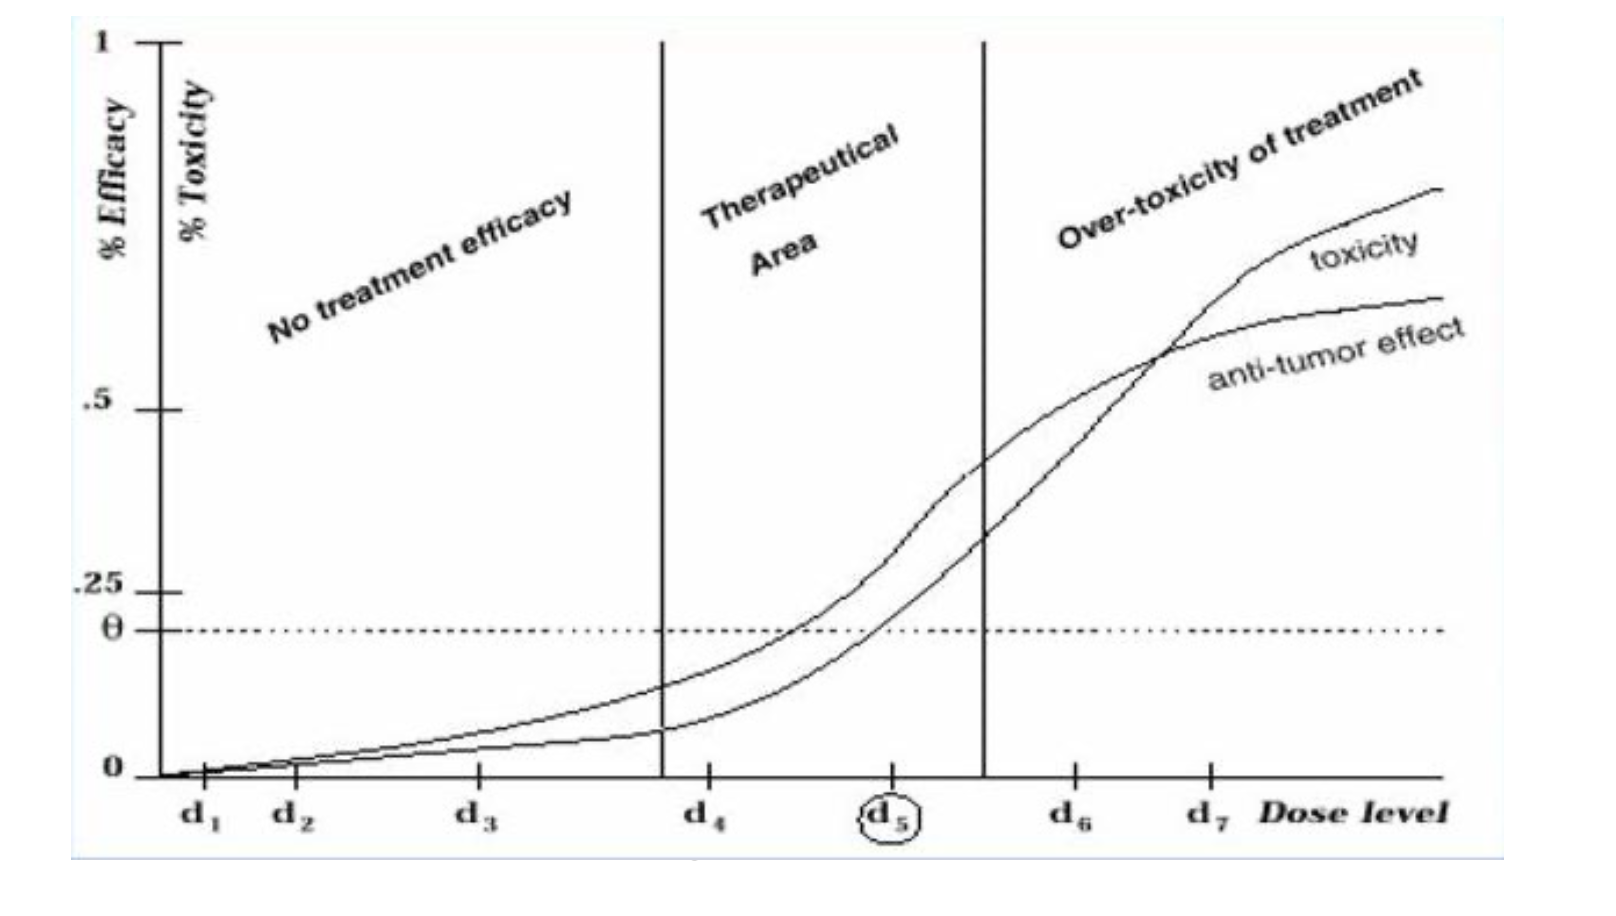
\includegraphics[scale=0.3]{images/paradignmedoseintensite.png}
    \caption{Paradigme "Dose-Intensité"}
    \label{fig:dose_intensite}
\end{figure}

La \textbf{Dose Limiting Toxicity [DLT]} est une occurrence d’une toxicité inacceptable
\begin{enumerate}
    \item  Pas de définition universelle – dépend de la pathologie considérée
    \item Doit être défini clairement dans le protocole. 
    \item Souvent définie en termes de CTCAE like in the Figure \ref{CTCAE}
\end{enumerate}

\begin{figure}[H]
    \centering
    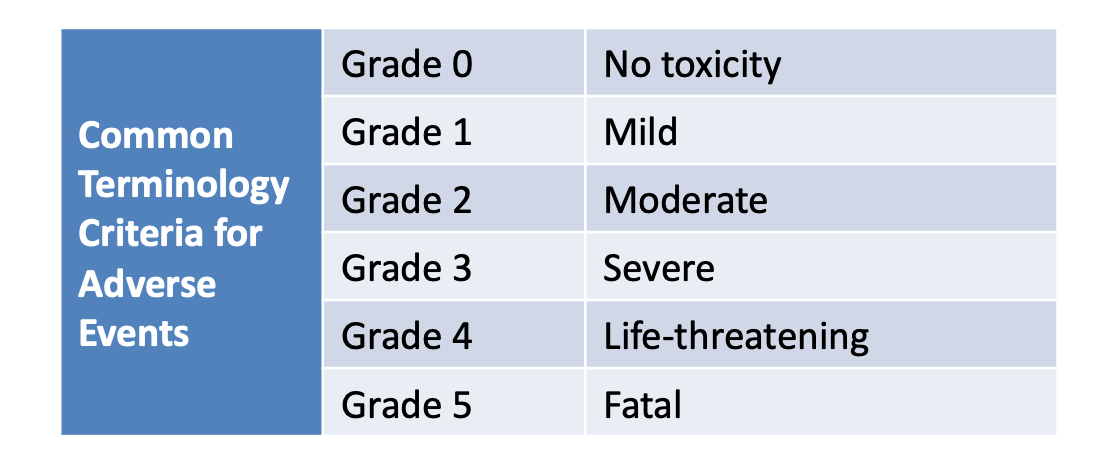
\includegraphics[scale =0.5]{images/CTCAE.png}
    \caption{CTCAE}
    \label{fig:CTCAE}
\end{figure}

\textbf{Dose maximum tolérée Maximum Tolerated Dose (MTD)} est la dose à laquelle la probabilité d’observer une DLT atteint un seuil donné.\\

La MTD est en général définie comme la proportion de cas de DLT :
$$Pr(DLT|MTD)=q_{0}$$

$q_{0}$ est généralement compris entre 0.1 et 0.4.\\

La MTD identifiée est ensuite utilisée comme dose de référence dans la suite du développement clinique (phase II).\\


\section{Contraintes}

\subsection{Contraintes pratiques}
seul un petit nombre de doses peuvent être observés par sujet. Cela a pour but d'éviter l'effet cumulatif des doses attribuées à un même patient, une longue période de « wash-out » étant en général pratiquement impossible.\\
Donc en général, une seule dose est testée sur chaque sujet.

\subsection{Contraintes éthiques}

On ne veut/peux pas exposer des patients à des doses associées à un niveau trop élevé de toxicité. On veut aussi éviter d'exposer des patients à des doses trop basses pour être efficaces. 

\section{Design}

\begin{figure}[H]
    \centering
    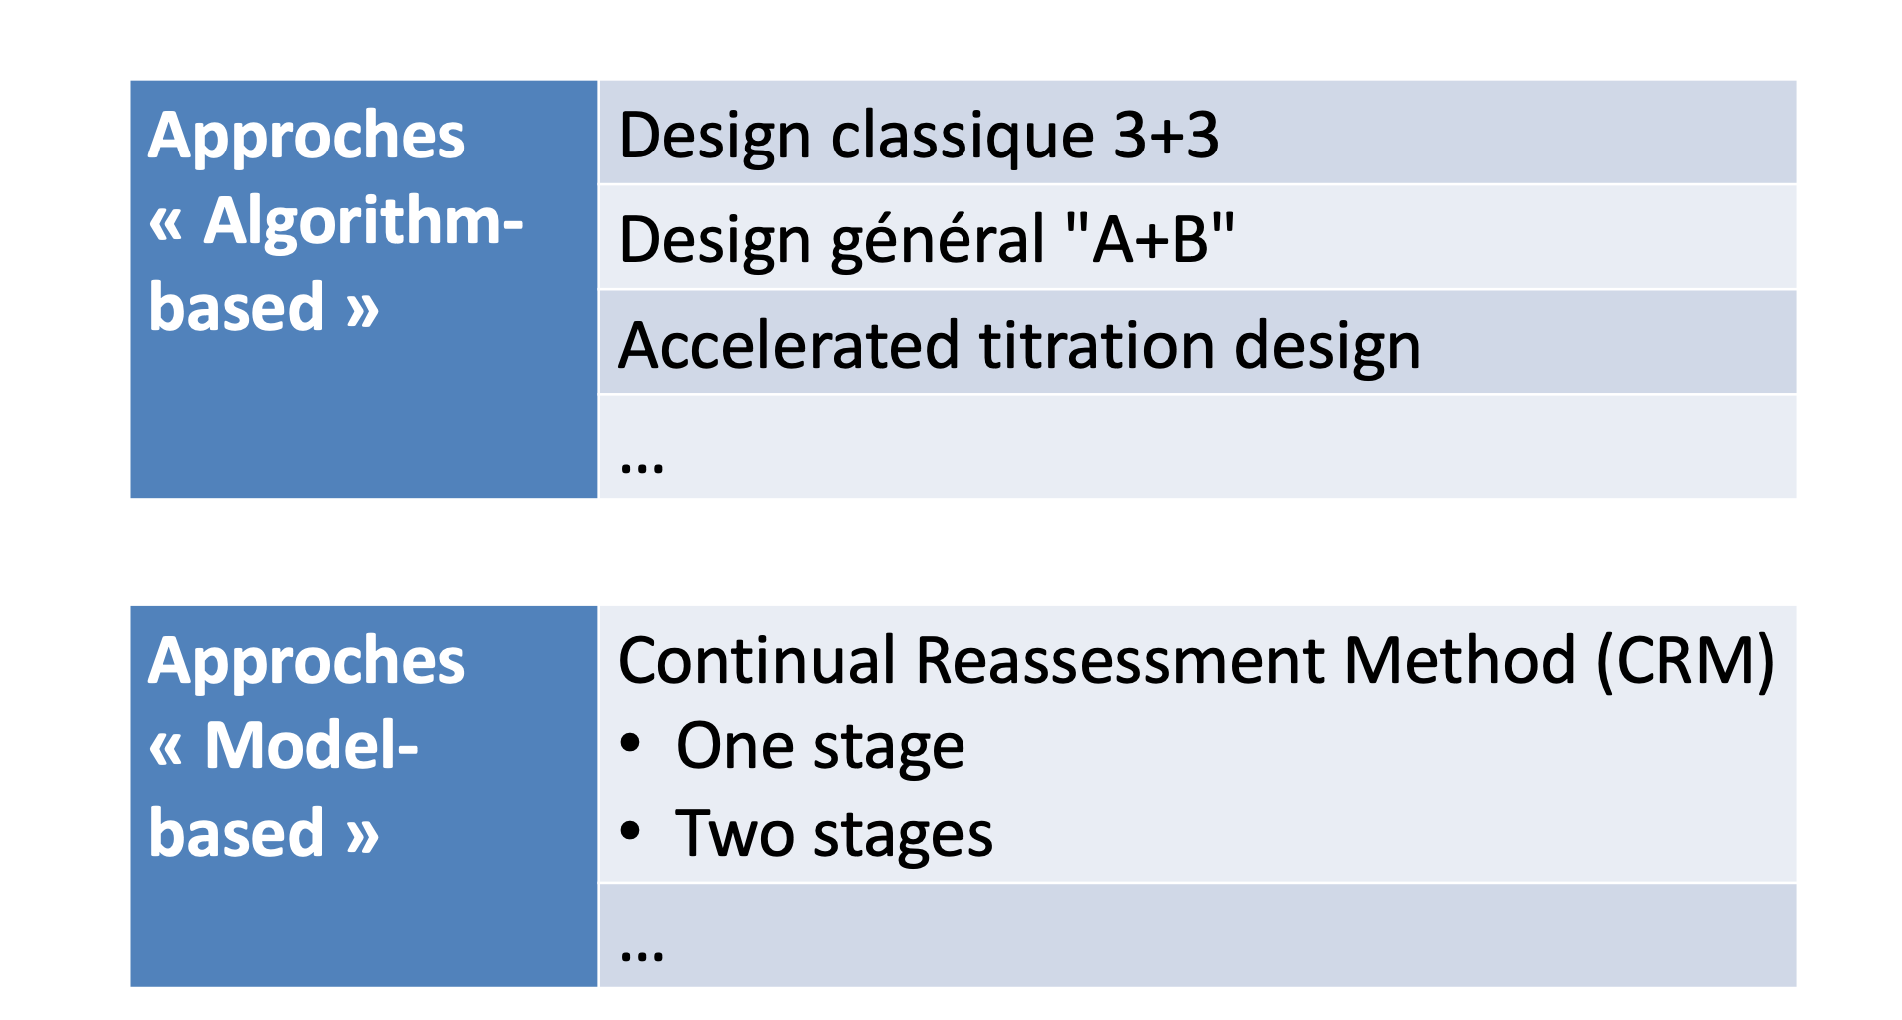
\includegraphics[scale=0.3]{images/designphase1.png}
    \caption{Différents designs en phase 1}
    \label{fig:designphase1}
\end{figure}

\subsection{Design classique 3+3}

\begin{figure}[H]
    \centering
    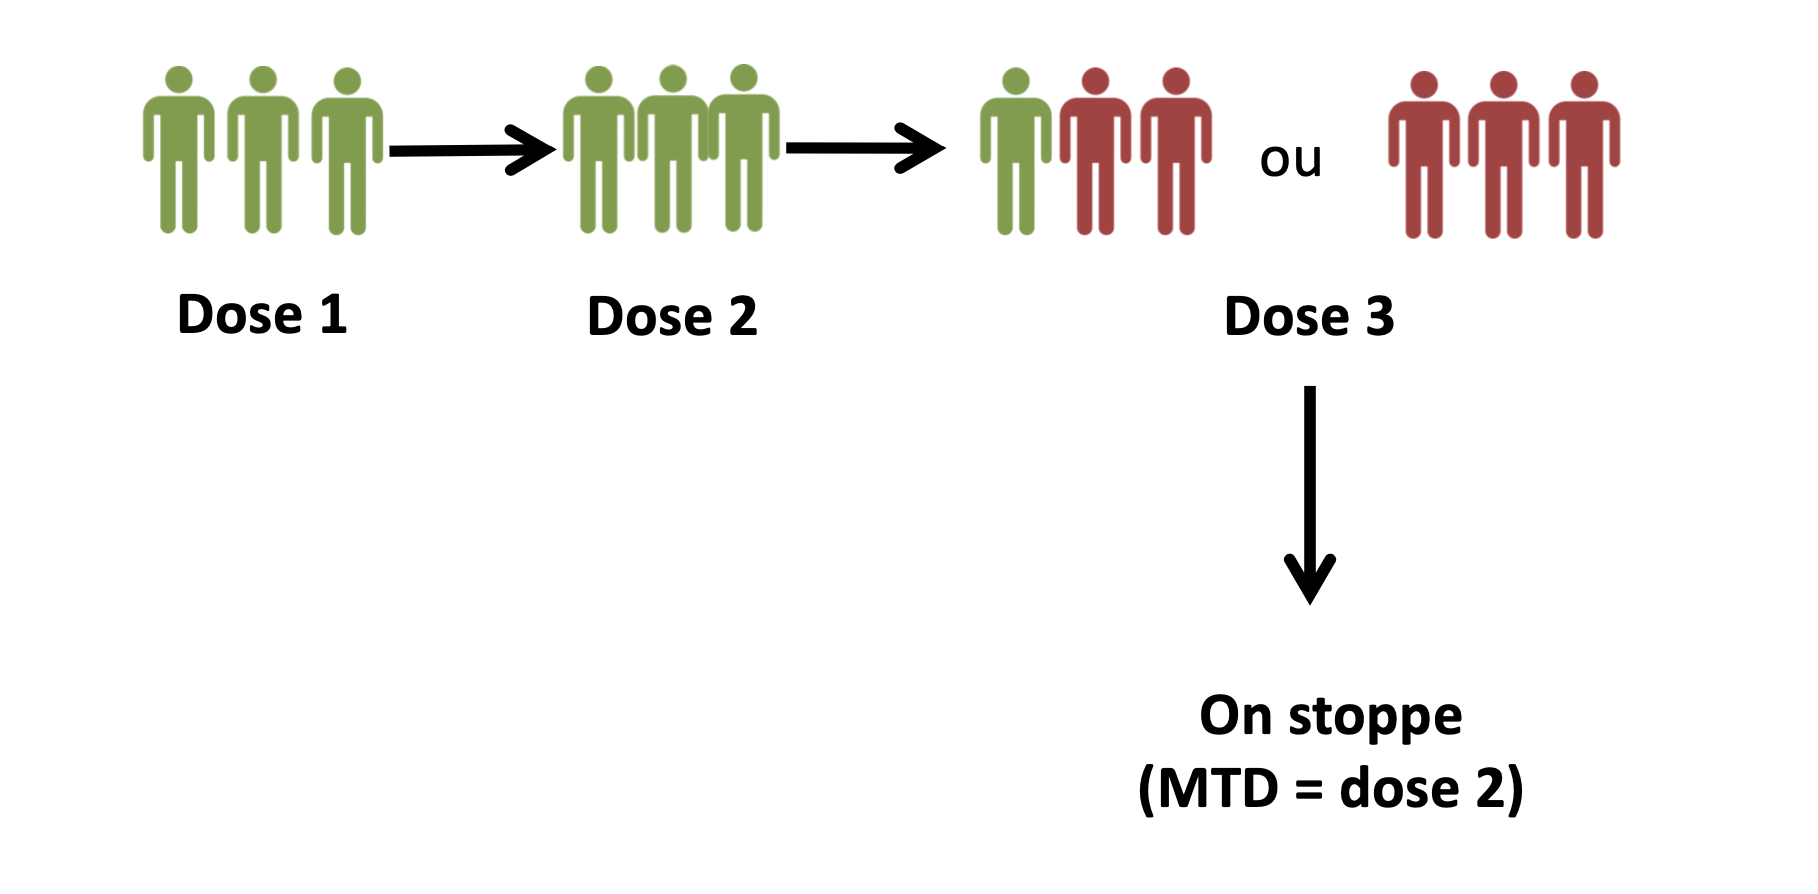
\includegraphics[scale=0.3]{images/3et31.png}
    \caption{Design 3+3}
    \label{fig:Design3et31}
\end{figure}

\begin{figure}[H]
    \centering
    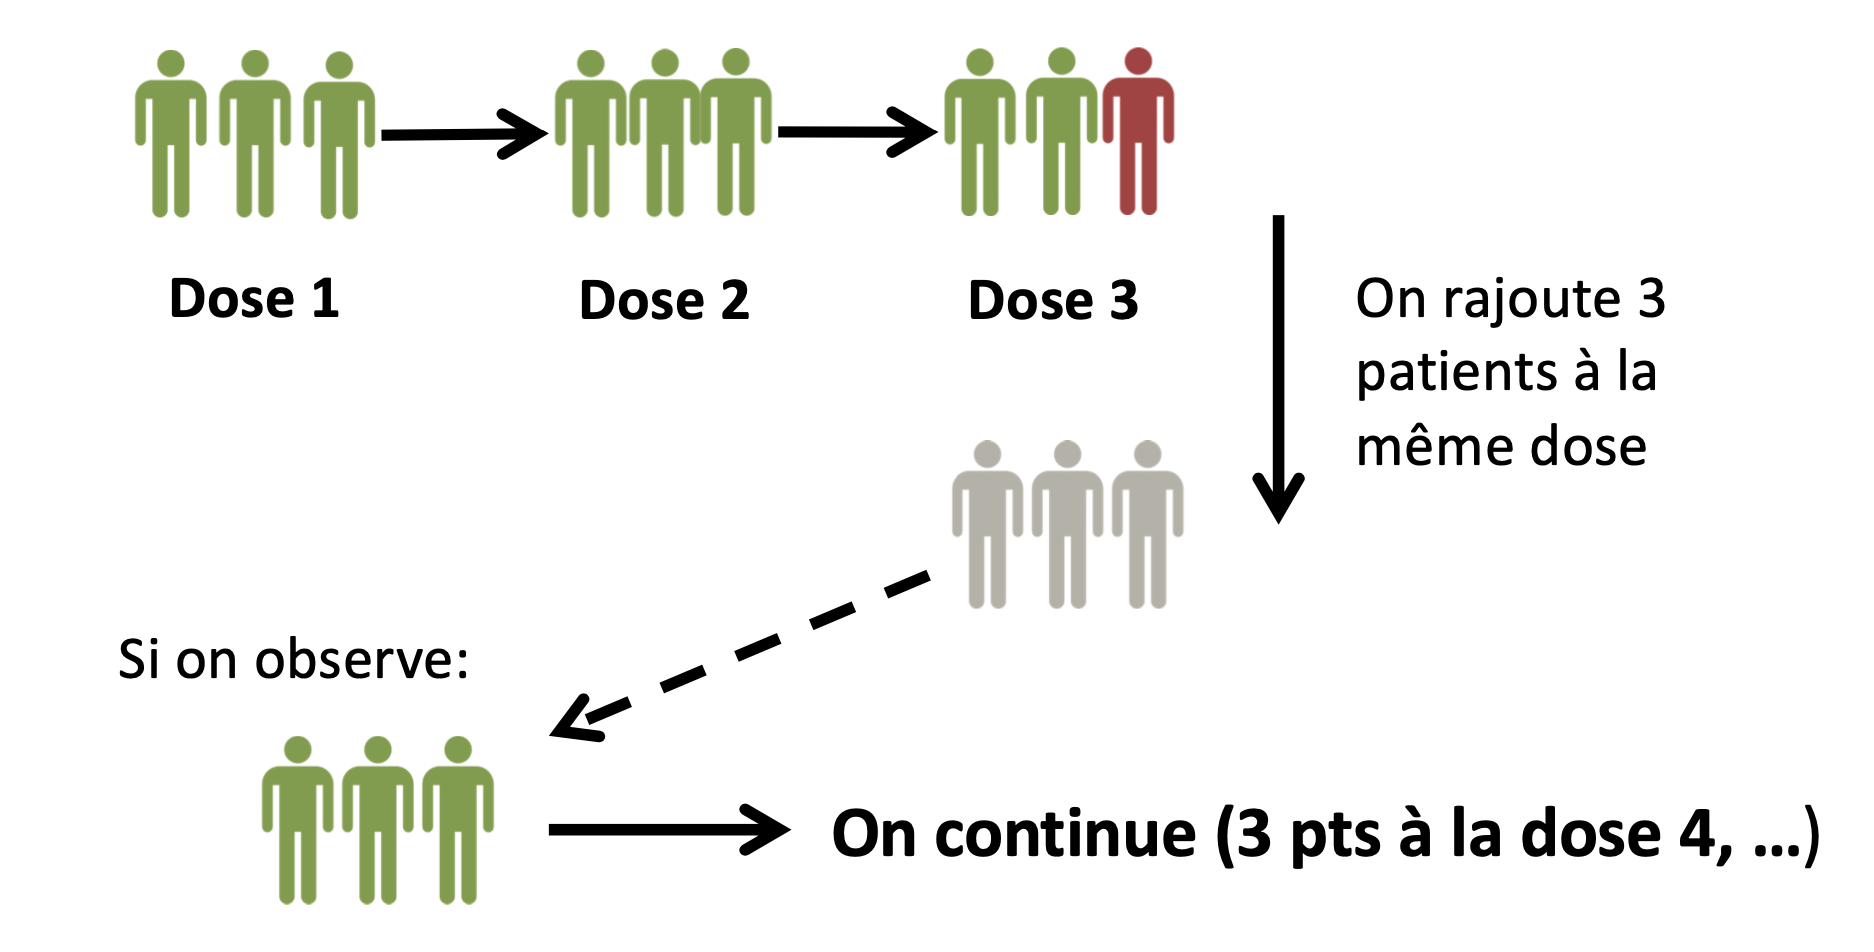
\includegraphics[scale=0.3]{images/3et32.png}
    \caption{Design 3+3}
    \label{fig:Design3et32}
\end{figure}

\begin{figure}[H]
    \centering
    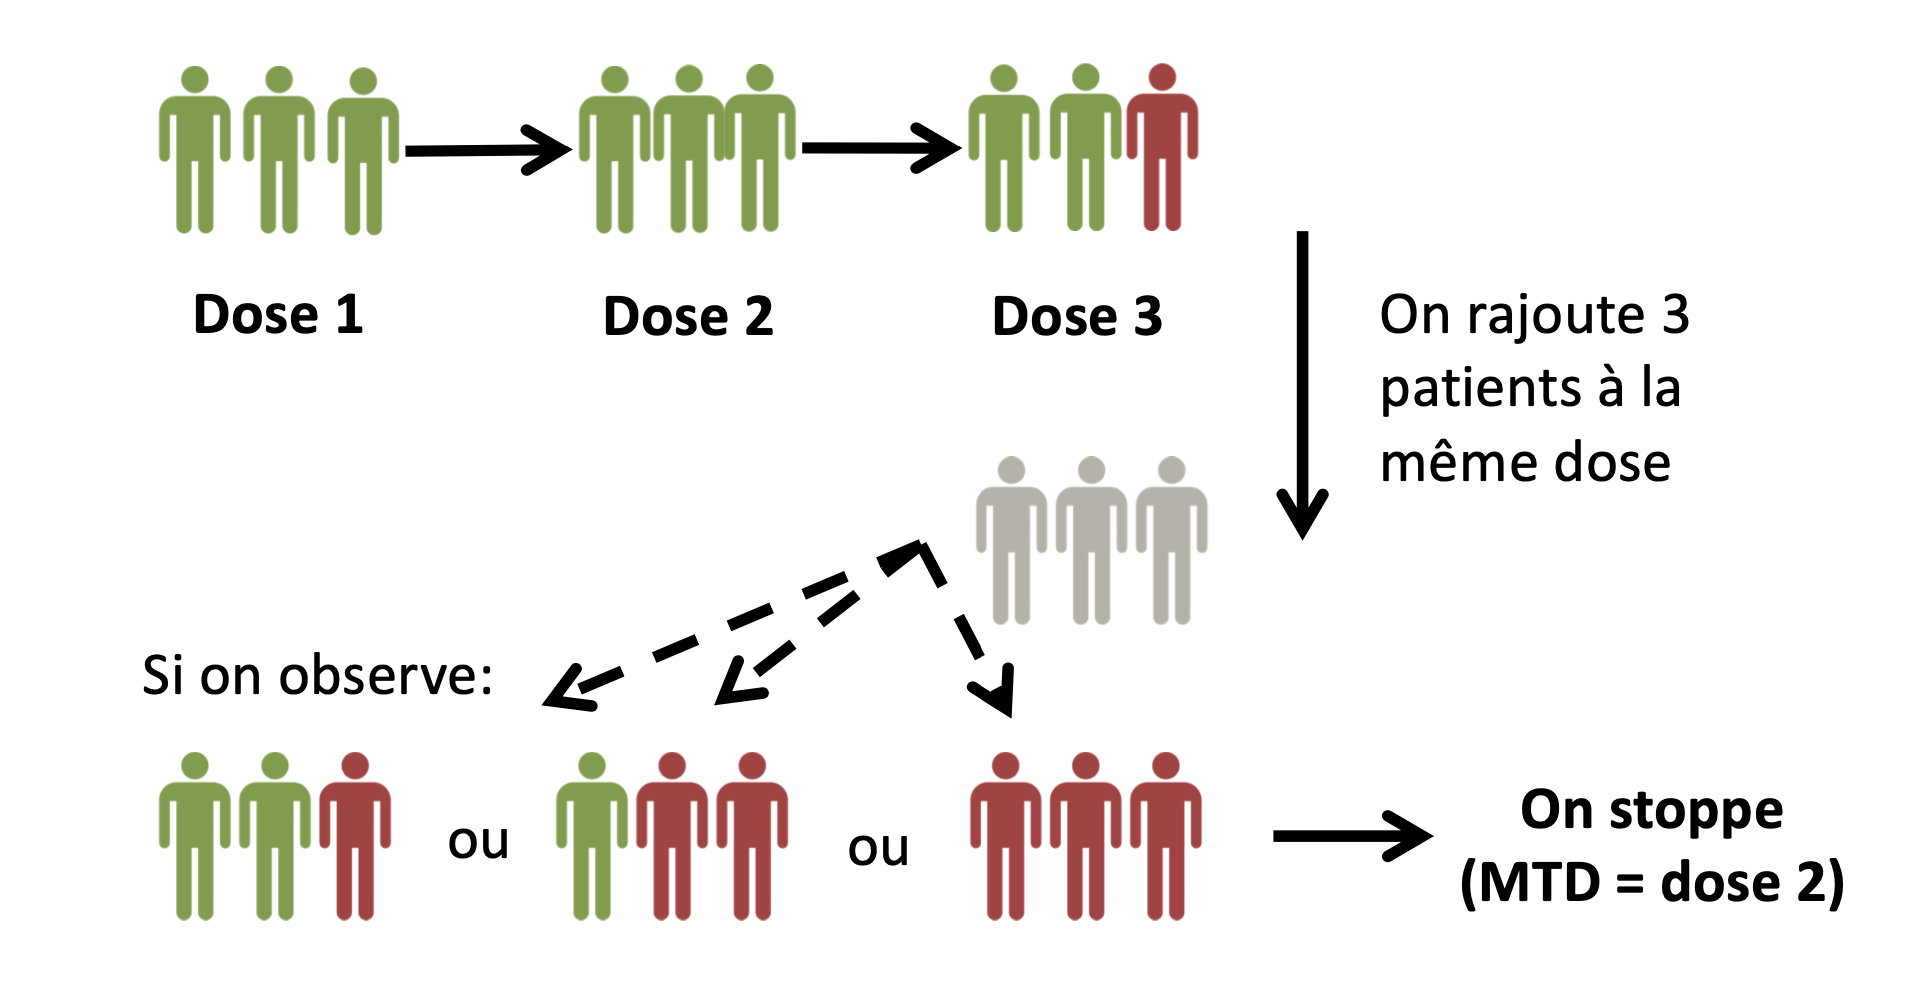
\includegraphics[scale=0.3]{images/3et33.png}
    \caption{Design 3+3}
    \label{fig:Design3et33}
\end{figure}
\subsubsection{Dose initiale $a_{1}$}
En général 1/10 de la $LD_{10}$(dose létale dans 10\% des souris traitées) pour la souris ajustée pour le poids. Pour les doses suivantes, on utilise des séquences mathématiques (Fibonacci, etc). 
\subsubsection{Inconvénients}
Cette méthode a des mauvaises propriétés statistiques.
\begin{figure}[H]
    \centering
    \includegraphics[scale=0.3]{}
    \caption{Statistique de 3+3}
    \label{fig:stat3+3}
\end{figure}
D'un point de vue statistique et éthique, on a une mauvaise utilisation de l’info. Seulement d'un point de vue éthique, cette méthode est très conservative et en pratique, c'est peu flexible.


\subsection{Continual Reassessment Method (CRM)}
Les objectifs de cette méthode sont de minimiser le nombre de pts traités à une dose trop faible ; de minimiser le nombre de pts traités à une dose trop haute ; de minimiser le nombre de pts total.

\subsubsection{Principes}
\begin{figure}[H]
    \centering
    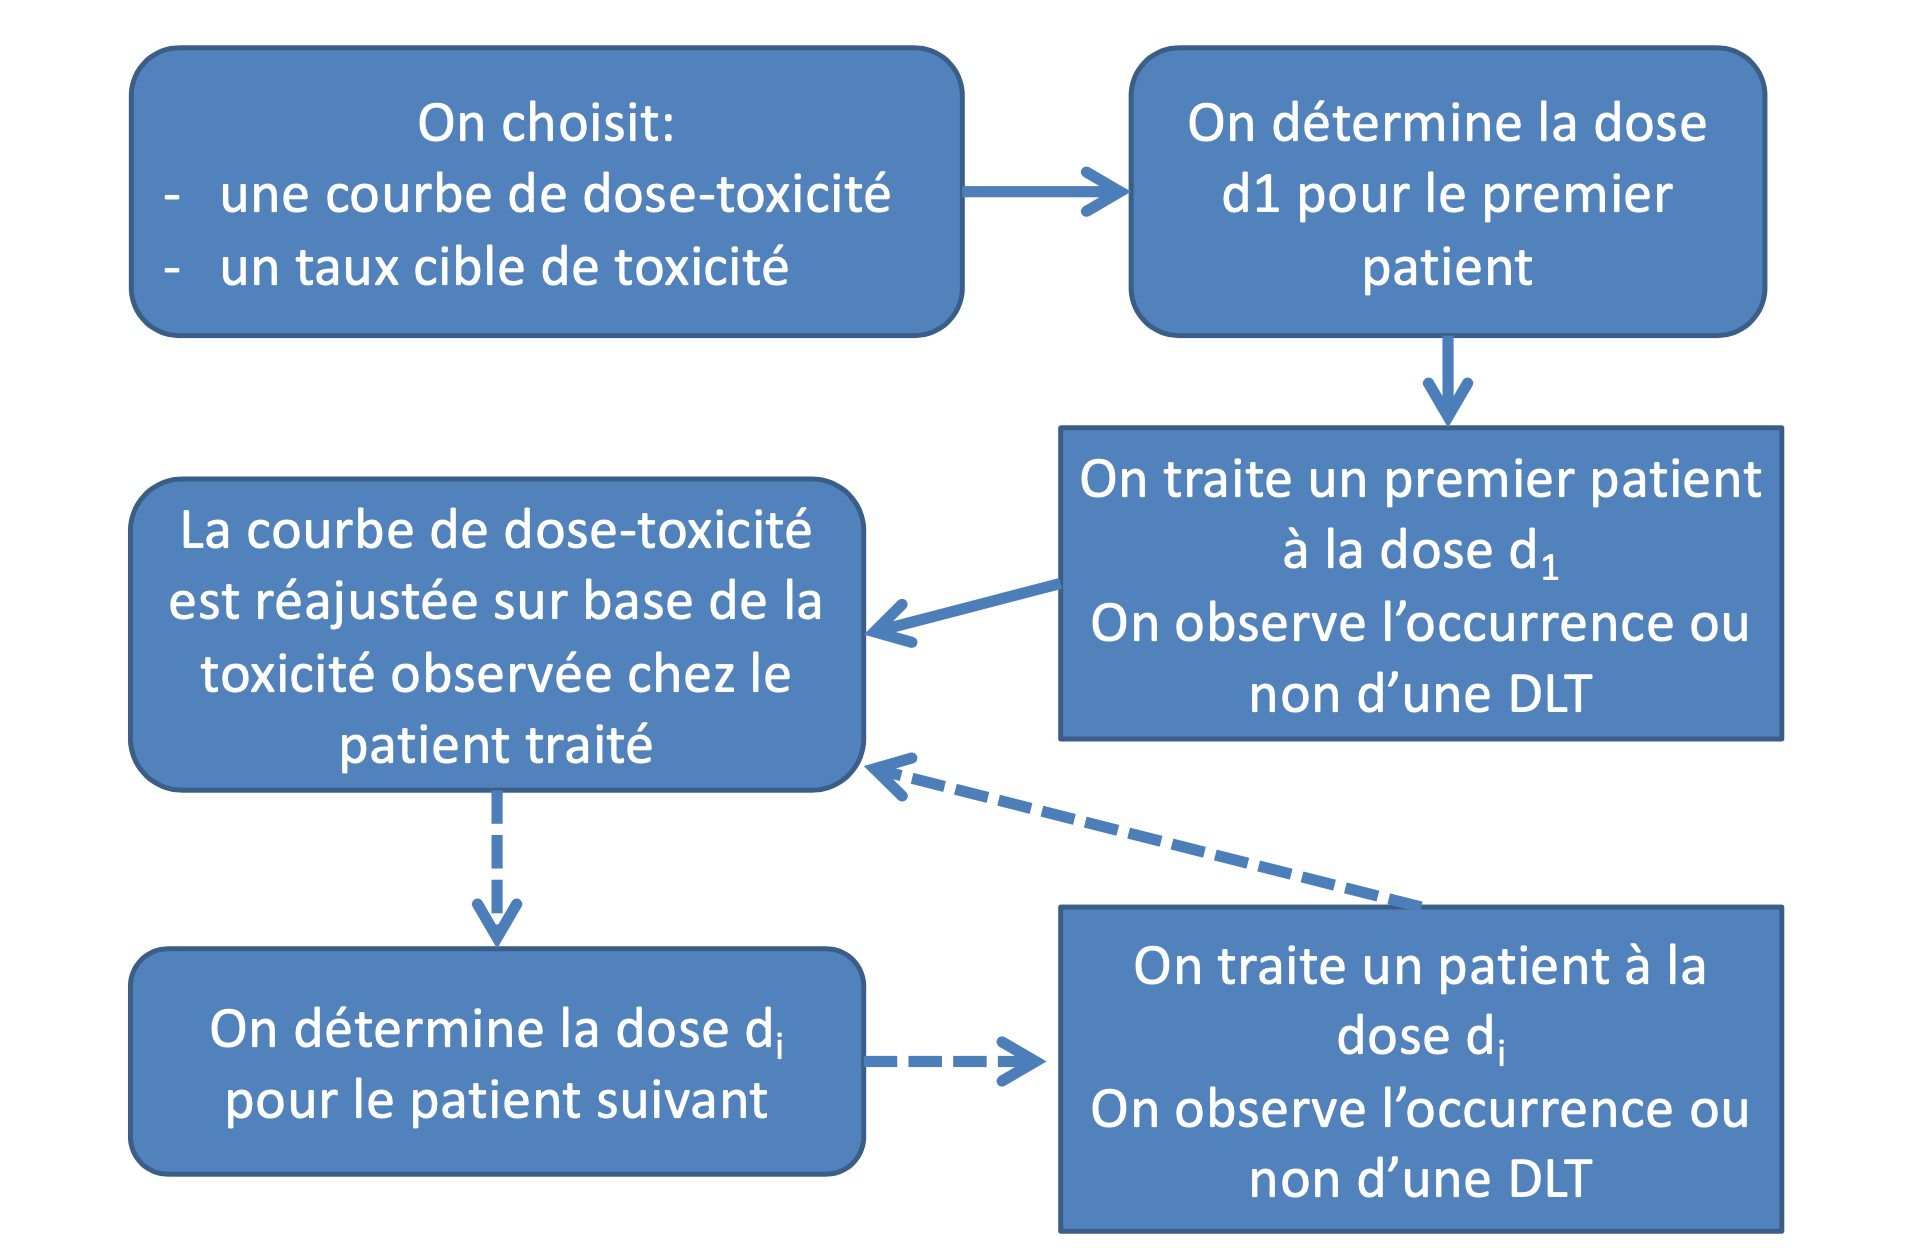
\includegraphics[scale=0.3]{images/CRM.png}
    \caption{CRM principe}
    \label{fig:CRMprincipe}
\end{figure}

\begin{figure}[H]
    \centering
    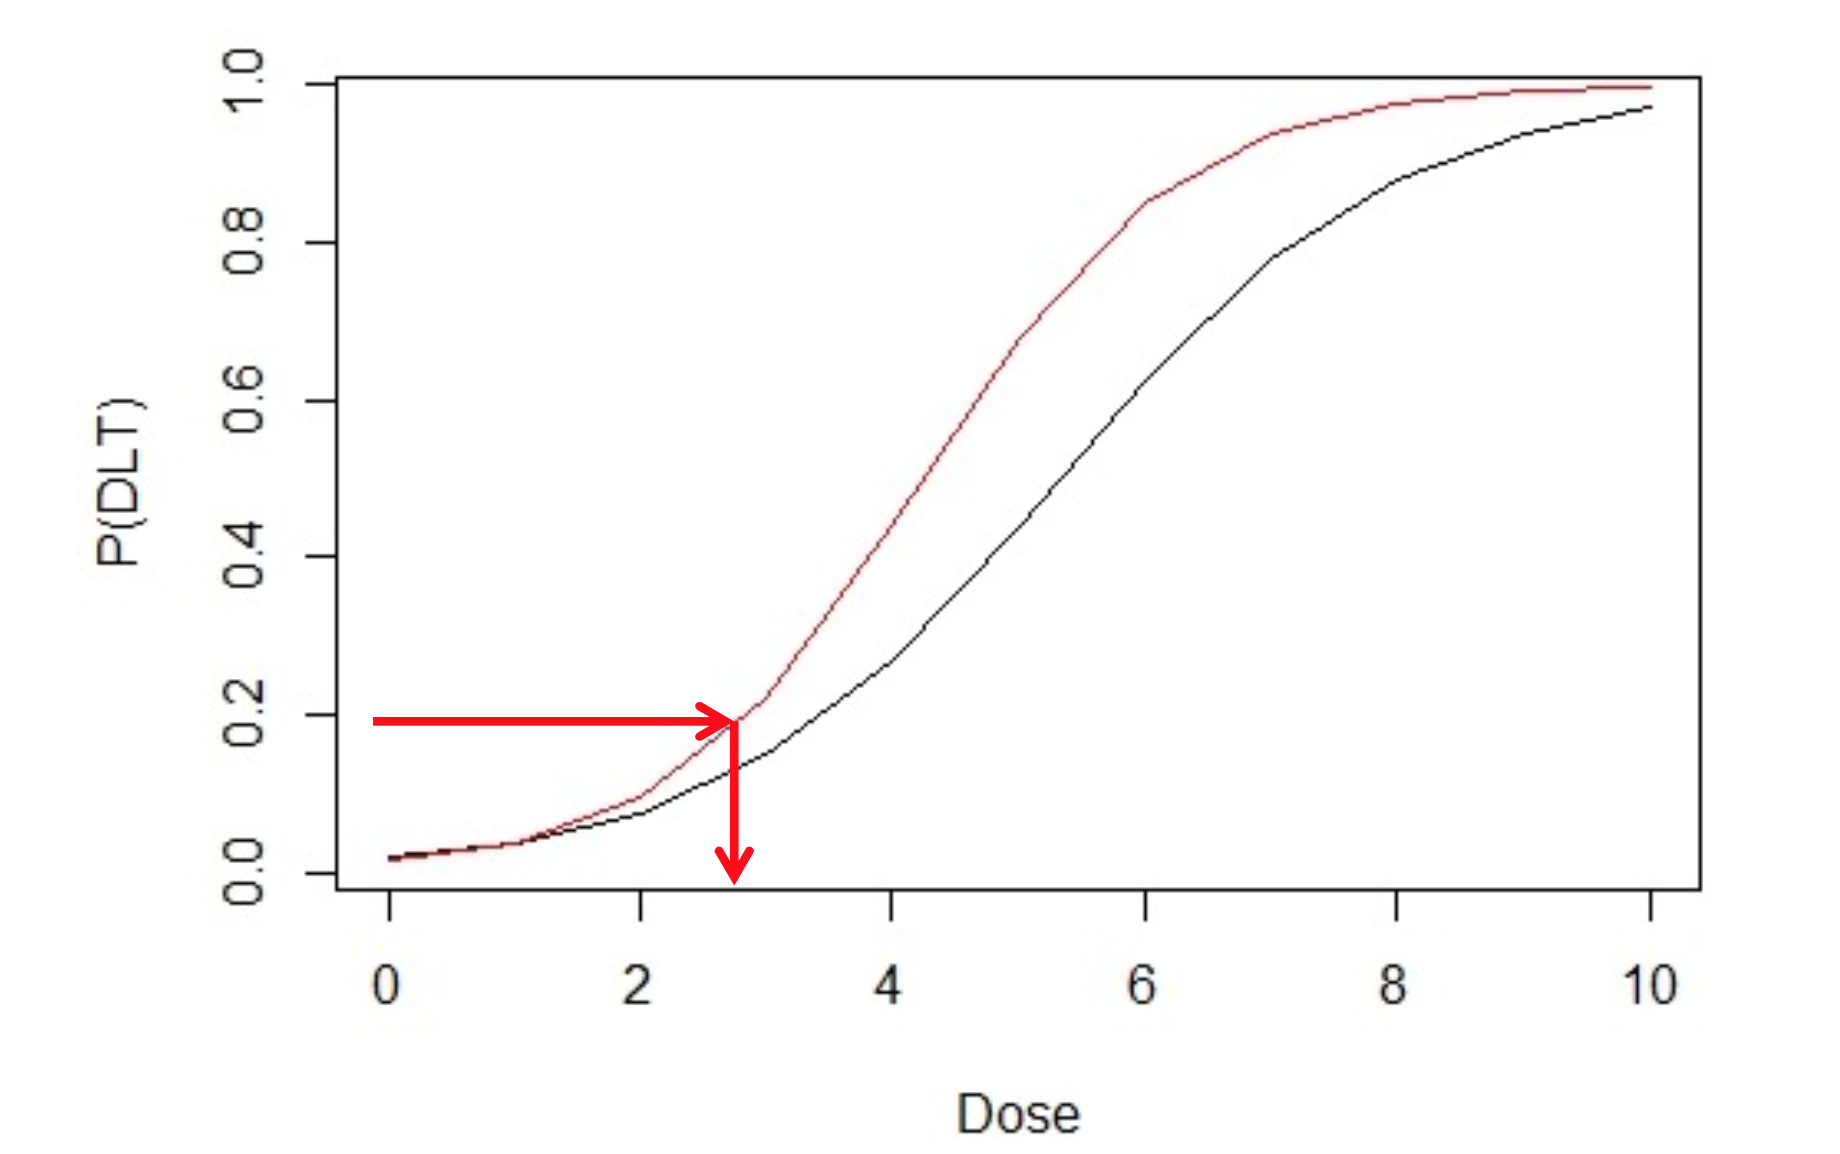
\includegraphics[scale=0.3]{images/CRMdose.png}
    \caption{Choix de la douse}
    \label{fig:CRMdose}
\end{figure}

\subsubsection{Choix de la courbe dose-toxicité}
Il existe différentes fonctions continues monotones : exponentielle, logistique, probit, ...\\
En général, on prend des fonctions à 1 ou 2 paramètres, car on a peu de données (la courbe autorisée à se modifier seulement sous un seul aspect (en général la pente)). 


\section{Remarques}

\begin{itemize}
    \item On n’est pas concerné par une estimation précise de toute la courbe de dose-toxicité, mais uniquement par son adéquation à proximité de la MTD
    \item Il a été démontré que la technique CRM est robuste pour la détermination de la MTD, même sous un choix de courbe de dose- toxicité modérément incorrecte.
\end{itemize}